%%%%%%%%%%%%%%%%%%%%%%%%%%%%%%%%%%%%%%%%%%%%
%% data section
%%%%%%%%%%%%%%%%%%%%%%%%%%%%%%%%%%%%%%%%%%%%
\section{Data exploration}
Understanding the historical data is crucial in forward simulation. 
We want to look at the data from many different angles and try to 
comprehend the relationships in them. This is not an easy task
given the scale of the data. This section will give some detailed
description of what I have learned from the data. 

\subsection{Natural Gas}
Being a major part of the portfolio, 
there are over 400 natural gas curves. 
Henry Hub gas price is the standard for
North America natural gas market so we will start 
from it. Figure \ref{henry-hist} shows historical prices of all
Henry Hub future contracts for past 200 days, with
each line representing a future contract. The top one plots 
in the original scale and the bottom figure plots prices 
centered around 0. We can see at the first glance that 
most of the curves are all very similar except for a few.
From the bottom figure one can see that the prices for
near futures have increased a lot while the prices for 
further futures stayed flat. As a result the curves crossed 
at around 130 days ago. This reflects the traders' view on natural
gas market. They think the natural gas price will increase in the
near future but drop back to normal after some time. Our 
simulation should reflect this trend. 
\begin{figure}[htbp]
\centering
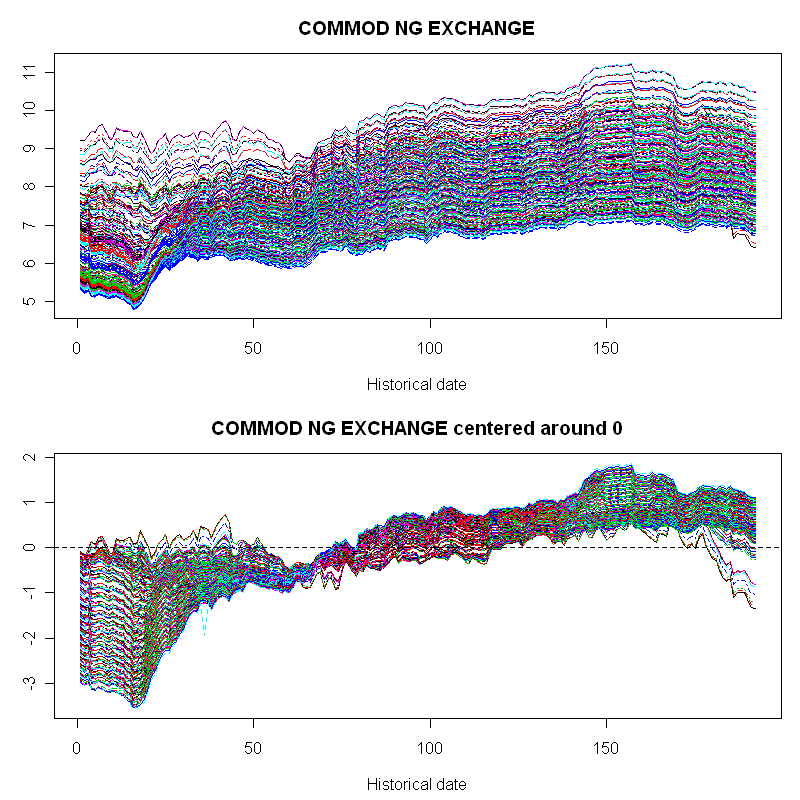
\includegraphics[width=4in, height=4in]{figures/henry01.png}
\caption{Historical prices for Henry Hub gas future.}
\label{henry-hist}
\end{figure}

Figure \ref{henry-hist-mon} 
shows the same plots, but for January and August contracts only.
The curves behaved similarly so the patterns are consistent
for all contracts. 
\begin{figure}[htbp]
\centering
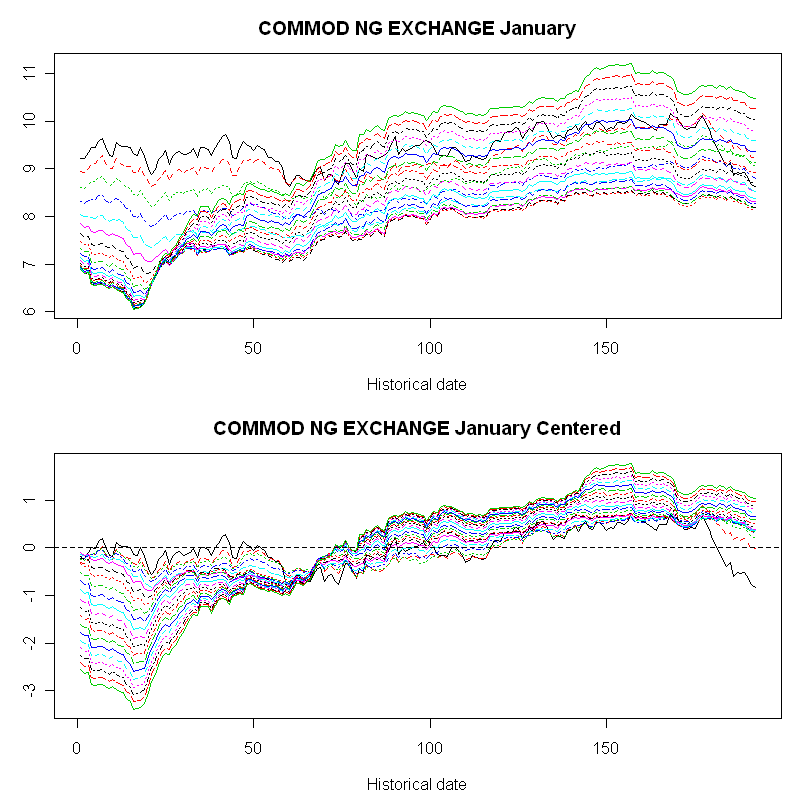
\includegraphics[width=4in, height=4in]{figures/henry02.png}
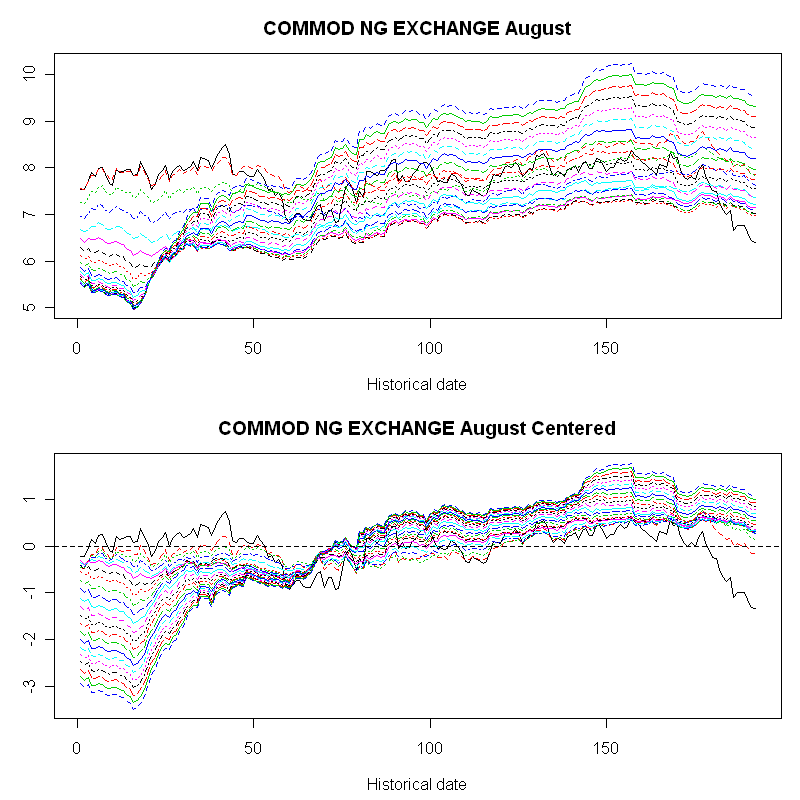
\includegraphics[width=4in, height=4in]{figures/henry03.png}
\caption{Historical prices for Henry Hub gas future - January
and August contracts only.}
\label{henry-hist-mon}
\end{figure}


Now look at the Henry Hub gas prices from another angle.
Figure \ref{henry-contract} plots the historical Henry Hub prices 
versus contract months. Each line represents a pricing day. 
The striking sinusodal pattern reflects the seasonality
and our simulation must capture this. The wide spread in the tail
reflects people's uncertainty of distant future. 
People orginally thought the gas price will increase 
in the future but changed their mind recently. Note that 
this change of future perspective depends on many 
factors such as new drilling, 
storage and pipeline construction, economic growth, etc.
It is very difficult to simulation solely based on 
historical prices. We can see later that our simulation
result shows very little of that, which suggests 
a more complex model might be necessary.

\begin{figure}[htbp]
\centering
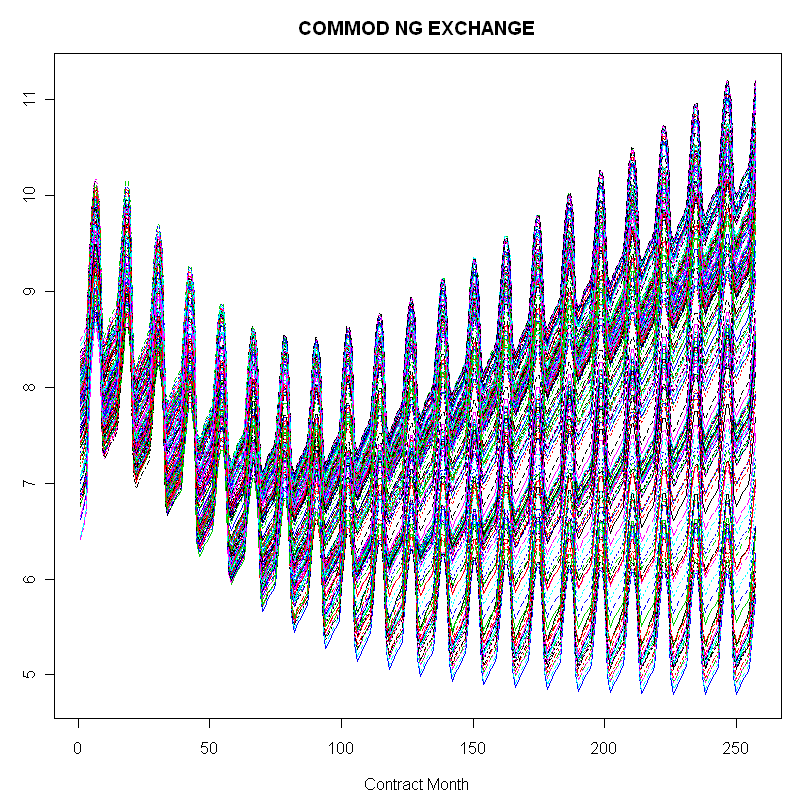
\includegraphics[width=3in, height=3in]{figures/henry04.png}
\caption{Henry Hub historical prices versus contract month.}
\label{henry-contract}
\end{figure}

Figure \ref{henry-contract-mon} shows the same plot
for January and August contracts. By taking the contract for a 
specific month we removed the seasonality. The up/down patterns
are preserved. 
\begin{figure}[htbp]
\centering
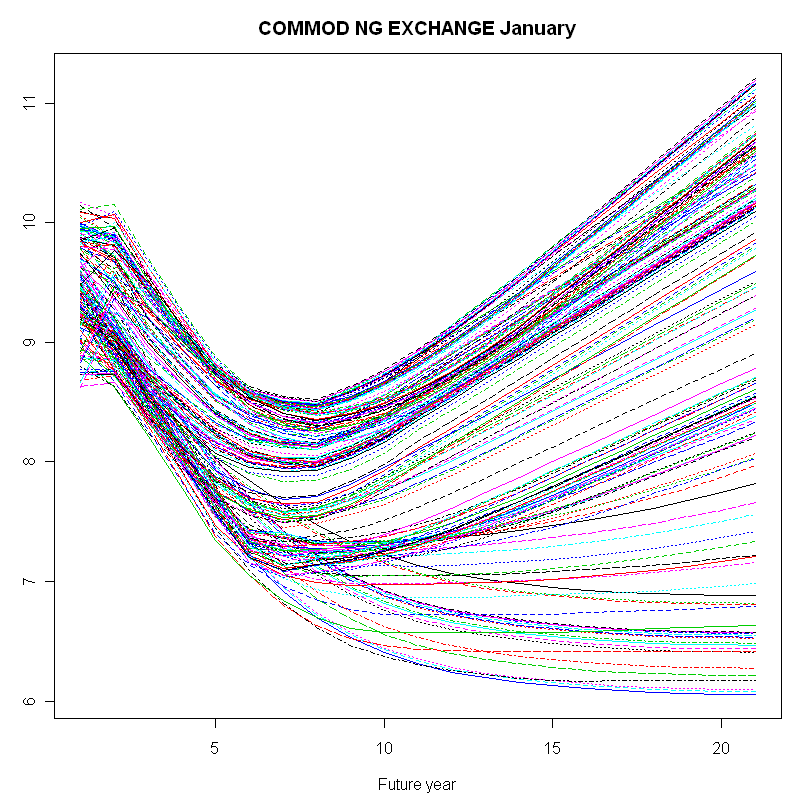
\includegraphics[width=3in, height=3in]{figures/henry06.png}
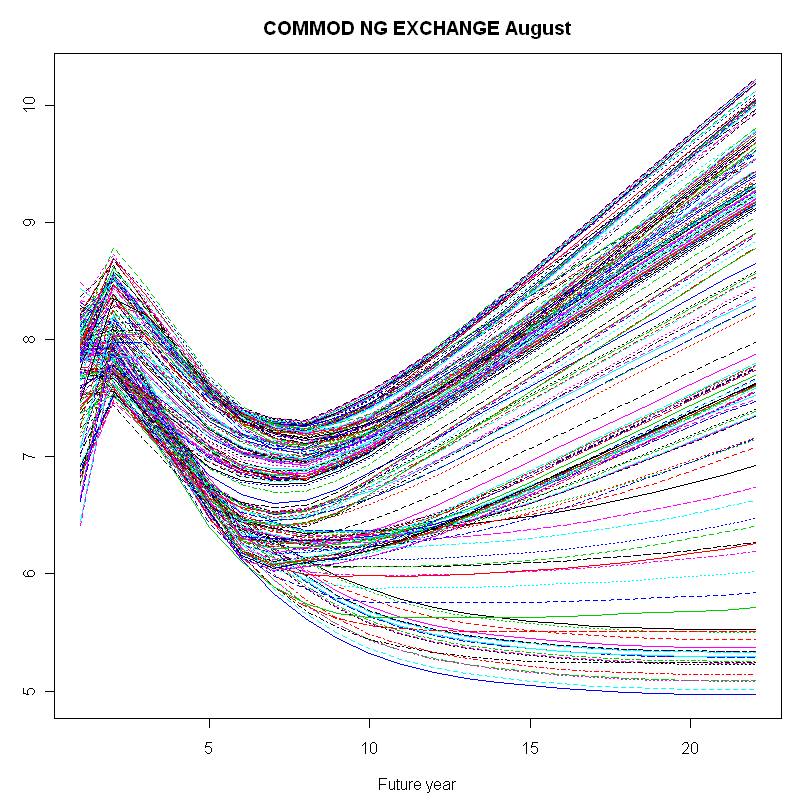
\includegraphics[width=3in, height=3in]{figures/henry05.png}
\caption{Henry Hub historical prices versus contract month -
January and August contracts only.}
\label{henry-contract-mon}
\end{figure}

Since we have observed from Figure \ref{henry-hist} that 
prices for all contract months are similary, we want to 
quantify the similarity by looking at their correlations. 
Figure \ref{henry-corr} shows the heat map for historical 
price correlations among future contracts. Darker means
less correlation. We can clearly see the correlations 
are above 0.9 for contracts in nearby months. The correlation
dropped to around 0.7 if two contracts are far apart, say, 
10 years. All correlations are above 0.9 for contracts 
10 years later. 
\begin{figure}[htbp]
\centering
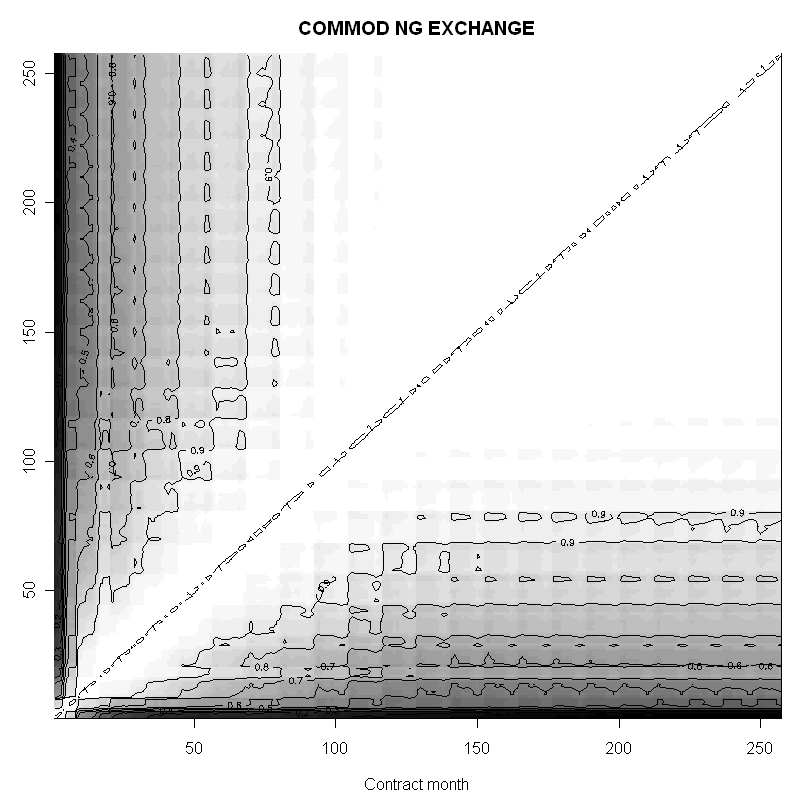
\includegraphics[width=3in, height=3in]{figures/henry07.png}
\caption{Henry Hub historical prices correlation among future contracts.}
\label{henry-corr}
\end{figure}

Now we want to look at curves at different locations. 
According to natural gas traders the whole North America
market can be divided into 17 regions. Each region has 
a leading curve. In figure \ref{ng-region-hist}, the left panel shows the 
historical prices of August 2007 contract 
for those 17 leading curves. We can see after centering
all curves are almost the same except for the one from
Rockie area. The right panel shows the correlation
among those prices. 
\begin{figure}[htbp]
\centering
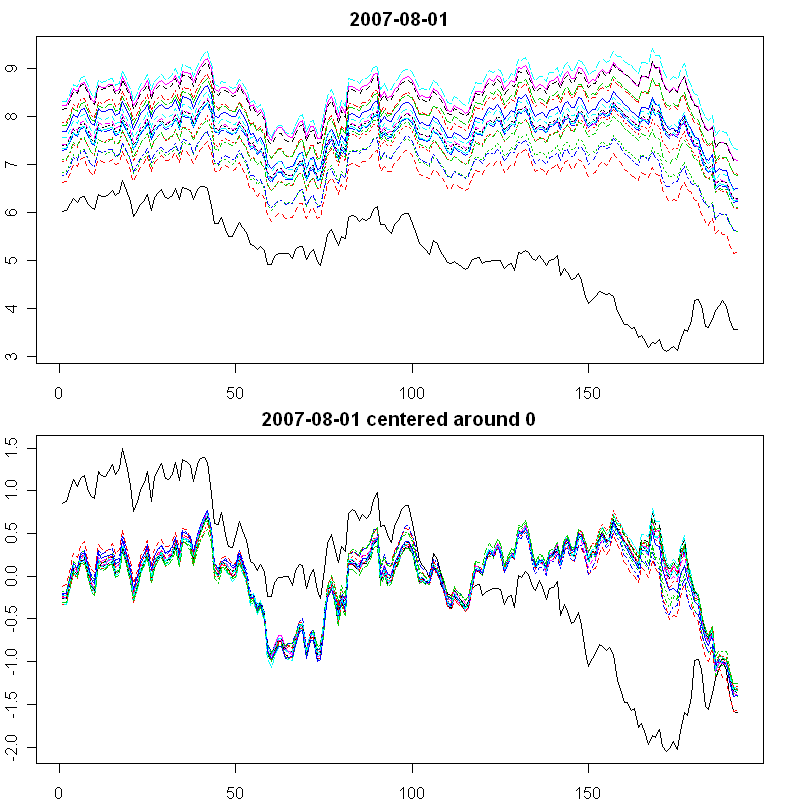
\includegraphics[width=3in, height=3in]{figures/regional-0708-01.png}
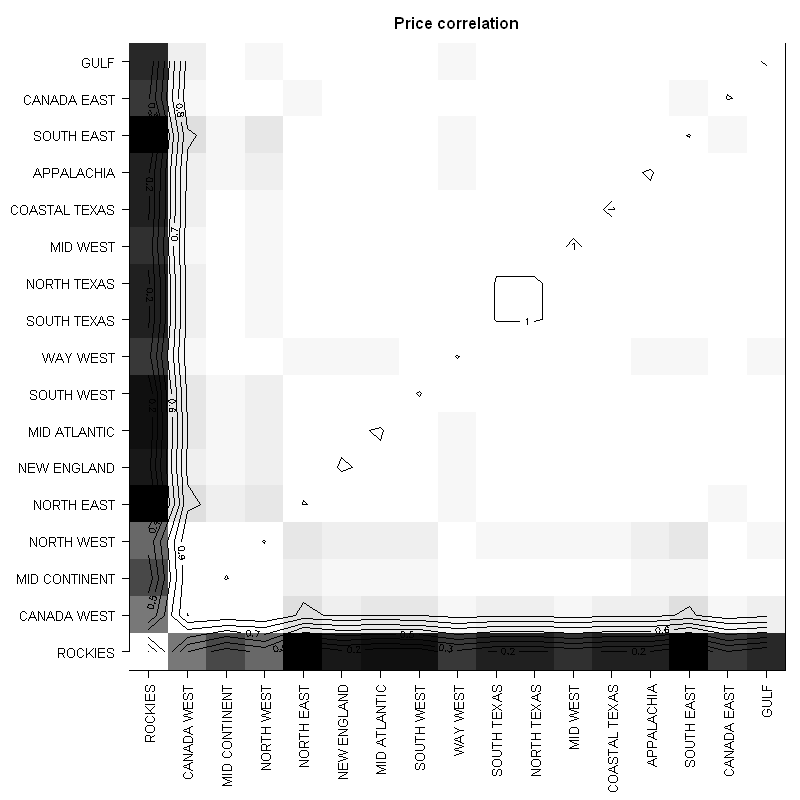
\includegraphics[width=3in, height=3in]{figures/regional-0708-02.png}
\caption{Historical prices of August 2007 contracts
for 17 regional leading curves. 
Left: Historical prices; Right: correlation among historical prices.}
\label{ng-region-hist}
\end{figure}


Figure \ref{ng-region-hclust} shows the hierarchical cluster 
for regional curves. The result shows that the markets physically close
were clustered together, which makes sense. 
\begin{figure}[htbp]
\centering
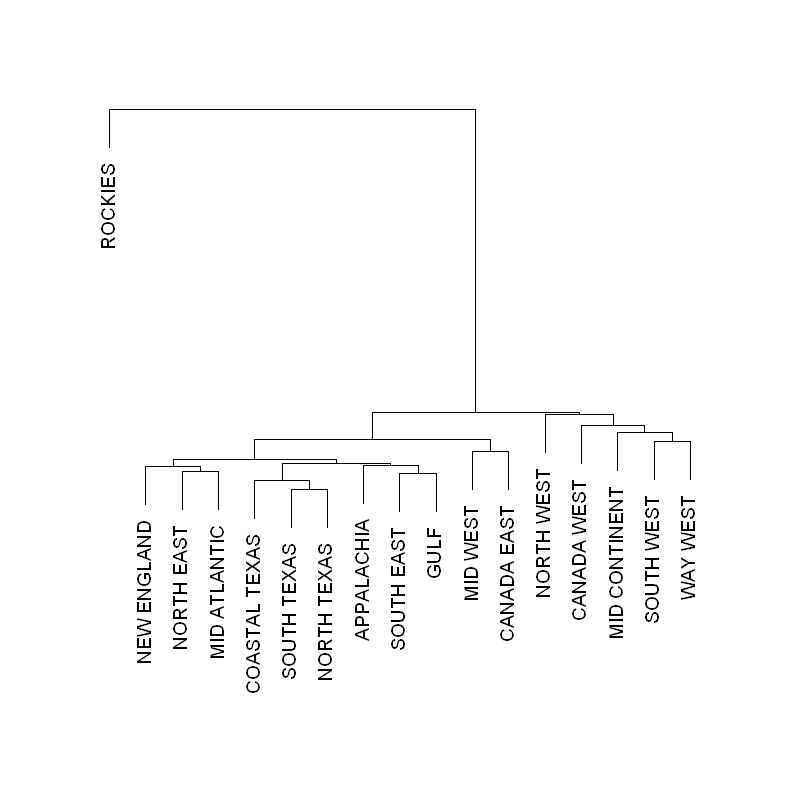
\includegraphics[width=3in, height=3in]{figures/regional-0708-04.png}
\caption{Hierarchical cluster on historical prices of August 2007 contract
for 17 regional leading curves.}
\label{ng-region-hclust}
\end{figure}

To summarize the findings in natural gas historical prices, we have:
\begin{enumerate}
\item For one curve, prices for all future contracts moved similarly.
\item Future contracts show seasonality, with the contracts for 
  January and August the most expensive.
\item For one contract month, all curves are very similar except
for those in Rockie Mountain area. 
\end{enumerate}

\subsection{Coal}
There are over 90 domestic coal curves. 
Figure \ref{col-hist} plots the historical prices of all
future contracts for COMMOD COL EXCHANGE, which is the standard
for domestic coal market. From the left panal
one can see that prices for all contracts 
are highly correlated, with the curves crossed a little bit. 
The right panel shows the prices by contract month.
Unlike the natural gas prices, there is no seasonality. 
The prices increase along with contract month, 
which means people think the coal price will increase 
in long term. 
\begin{figure}[htbp]
\centering
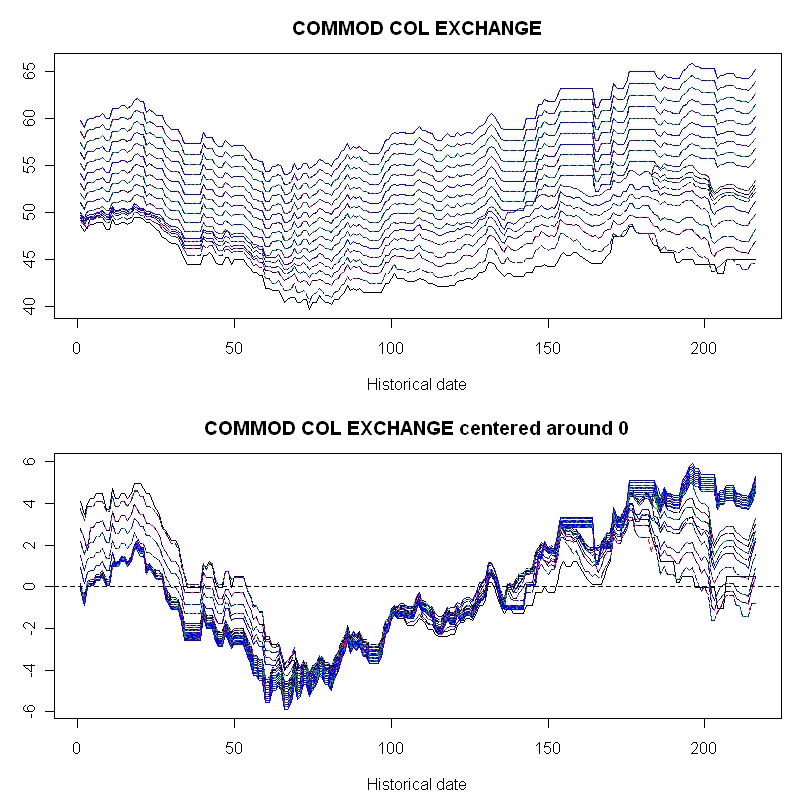
\includegraphics[width=3in, height=3in]{figures/col01.png}
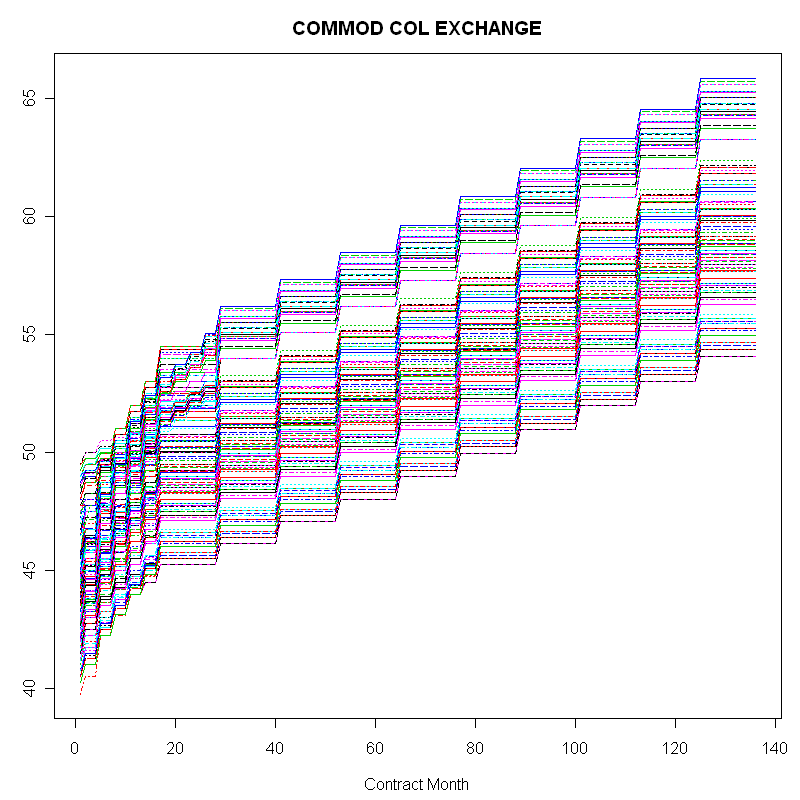
\includegraphics[width=3in, height=3in]{figures/col02.png}
\caption{Historical prices for COMMOD COL EXCHANGE. 
Left: prices for all future contracts. 
Right: Prices versus contract months.}
\label{col-hist}
\end{figure}


\subsection{Crude Oil}
There are only 8 Oil curves (WTI). 
Figure \ref{wti-hist} plots the historical prices of all
future contracts for COMMOD WTI EXCHANGE,  the standard
for crude oil market. Again from the left panal
one can see that prices for all contracts 
are highly correlated.
The right panel shows the prices by contract month.
There's no seasonality and the prices are almost
flat along with future months, which means people currently
think the long term crude oil price won't change much.

\begin{figure}[htbp]
\centering
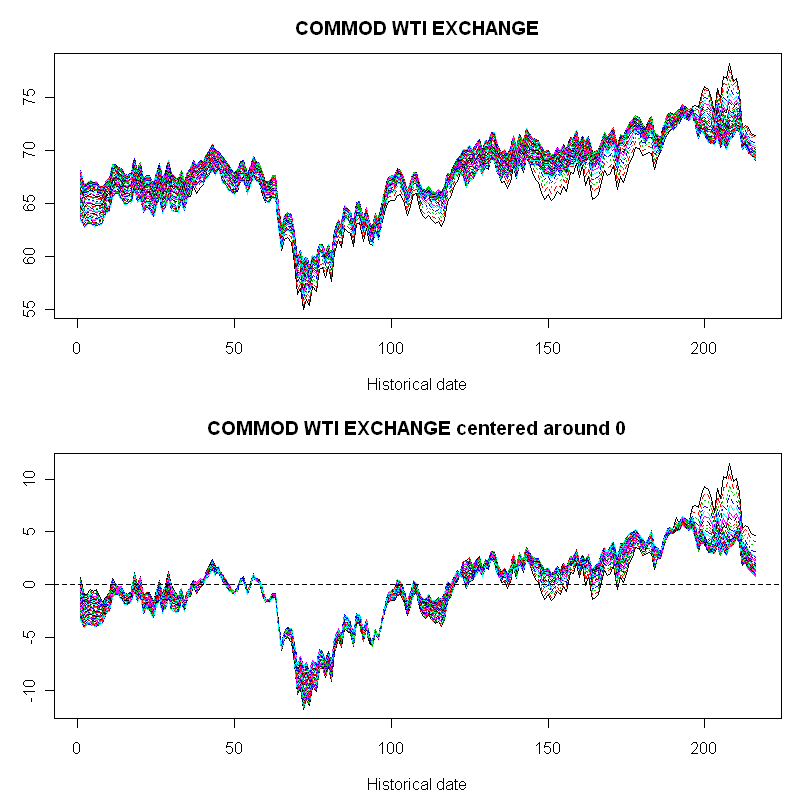
\includegraphics[width=3in, height=3in]{figures/wti01.png}
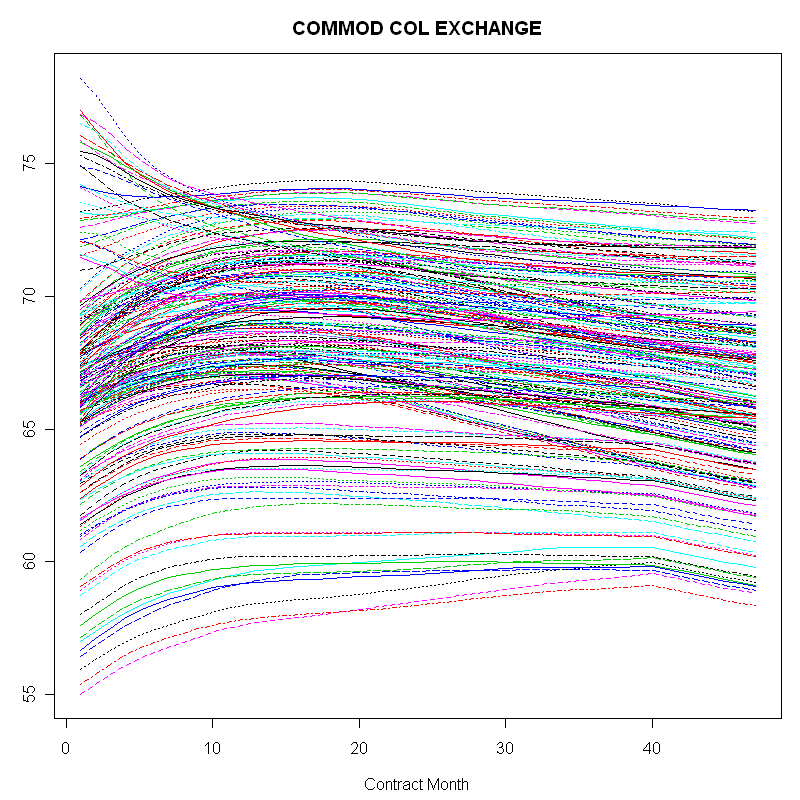
\includegraphics[width=3in, height=3in]{figures/wti02.png}
\caption{Historical prices for COMMOD WTI EXCHANGE. 
Left: prices for all future contracts. 
Right: Prices versus contract months.}
\label{wti-hist}
\end{figure}

\subsection{All fuels}
We want to understand the relationship among different 
types of fuels. We took three fuel exchange curves, 
shifted and rescaled the historical prices to make them 
have the same mean and standard deviation.
Figure \ref{allfuel} shows the three transformed  prices for 
for September 2007 contract. 
One can see these prices are mildly correlated 
with correlation coefficient being around 0.5. 
\begin{figure}[htbp]
\centering
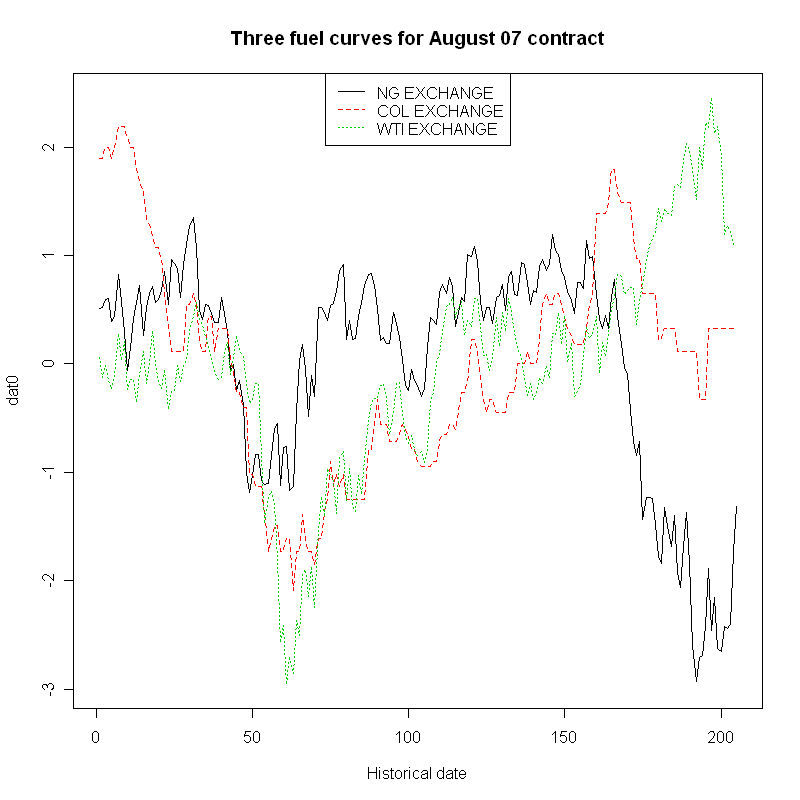
\includegraphics[width=3in, height=3in]{figures/allfuels.png}
\caption{Historical prices (shifted and scaled) of
three major fuel curves.}
\label{allfuel}
\end{figure}

\subsection{Electricity}
There are around 20 regional electricity markets in North America
and part of Europe. Each market could have as many as 400+ 
curves (such as PWY), or as little as less than 10 curves 
(such as PWF). Totally there are close to 2000 curves 
so the scale of the data is huge. 

Figure \ref{pwy-hist} shows the historical prices of
all future contracts for one of
the major PWY peak hour curves. Left panel shows the 
daily price changes and right panel shows the prices
versus contract months. We can see that (1) the prices
for different contract are still very similar, although
the correlation is lower than those in natural gas;
and (2) Electricity prices show seasonalities with the prices
in summer higher than the prices in winter (note that month 0 is
August). 
\begin{figure}[htbp]
\centering
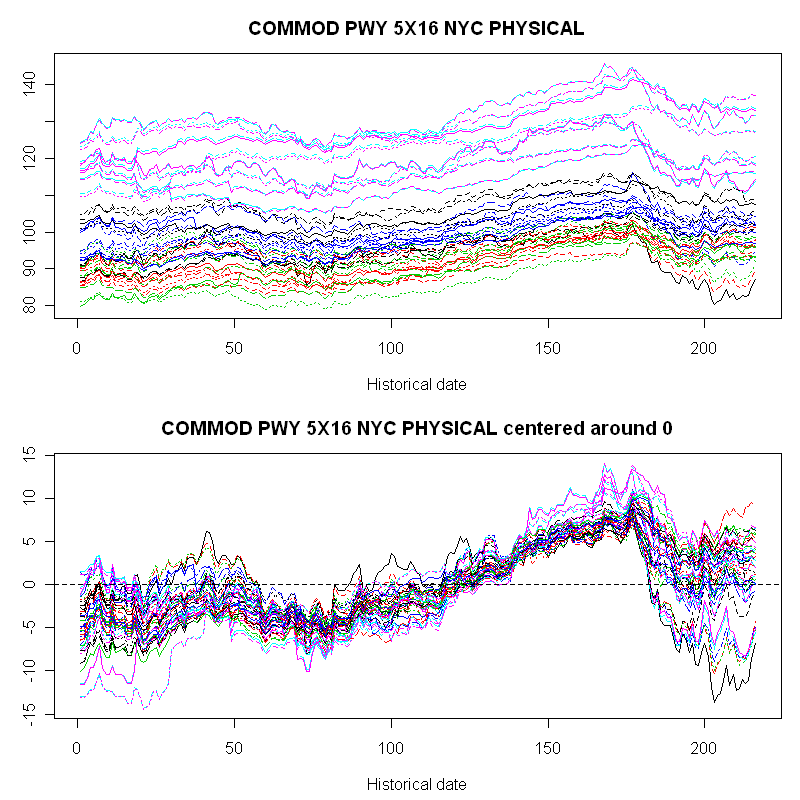
\includegraphics[width=3in, height=3in]{figures/pwy01.png}
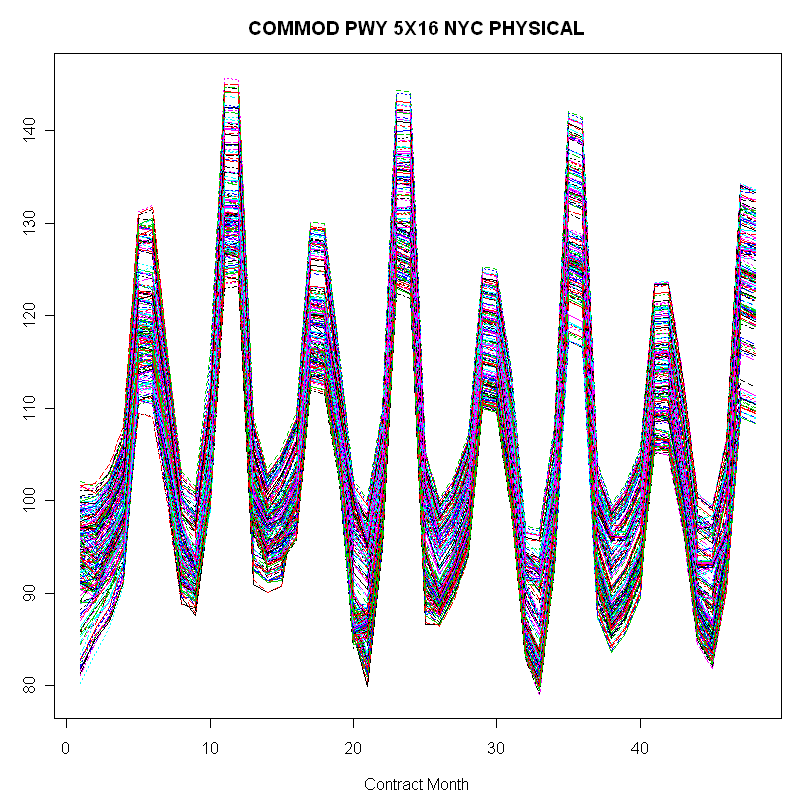
\includegraphics[width=3in, height=3in]{figures/pwy02.png}
\caption{Historical prices for COMMOD PWY 5X16 NYC PHYSICAL.
Left: prices for all future contracts. 
Right: Prices versus contract months.}
\label{pwy-hist}
\end{figure}

Figure \ref{pwy-contract} shows all PWY curves for the same contract month.
They are very similar but the similarity is not as strong as in natural
gas data. 
\begin{figure}[htbp]
\centering
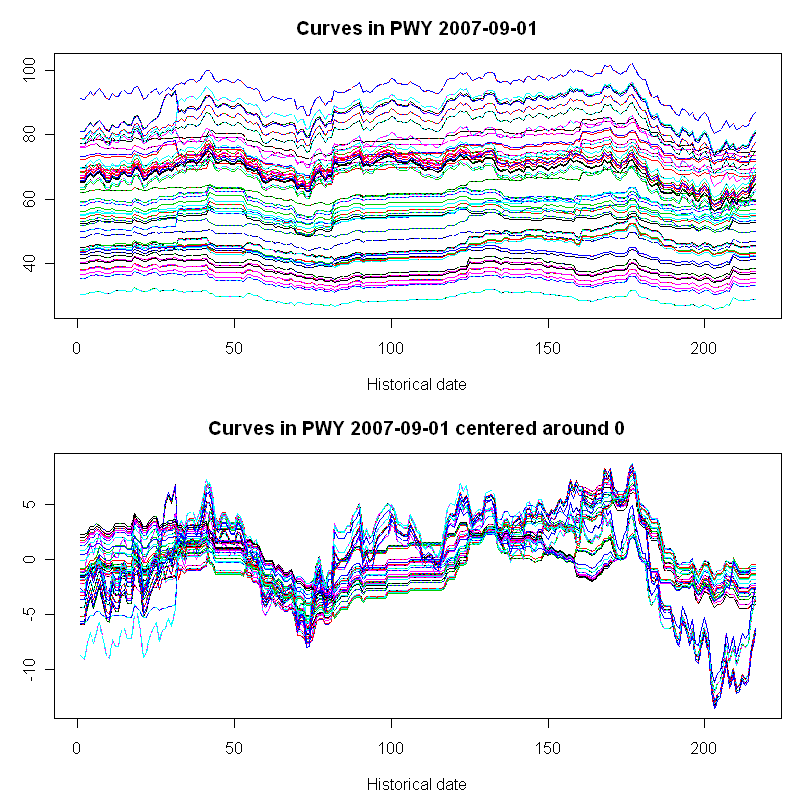
\includegraphics[width=3in, height=3in]{figures/pwy-contract.png}
\caption{Historical prices for all curves in PWY, September 2007 contract.}
\label{pwy-contract}
\end{figure}

In order to find the group structure in electricity prices, 
We did K-means clustering on PWY data. The result shows that
data can be roughly clustered into 2 or 3 groups. 5X16
curves show great similarity and always grouped together,
so are the 7X8 curves. 2X16 curves floats between these two groups,
depending on  market location and contract month.
I guess that that the grouping depends on many other factors
such as demand, fuel prices, etc. The grouping is not very 
important in forward curve simulation so in order to simplify it, 
we divide the electricity curves into peak and offpeak groups
and put 2X16 into the peak groups. 
Figure \ref{pwy-kmean} shows a K-mean clustering result of 2 groups
for PWY September 2007 conract. The figure at top are roughly 
the offpeak curves and the one at bottom are peak curves.
\begin{figure}[htbp]
\centering
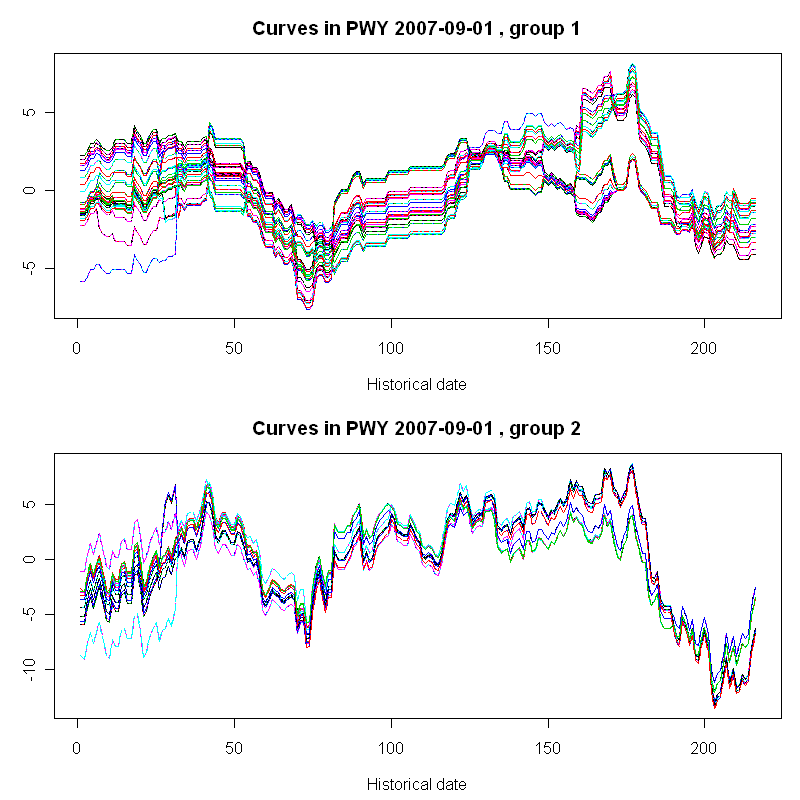
\includegraphics[width=3in, height=3in]{figures/pwy-kmeans.png}
\caption{K-mean clusters of PWY historical prices for September 2007 conract.}
\label{pwy-kmean}
\end{figure}


Now we want to explore the relationship between electricity 
and fuel prices. Figure \ref{pwy-fuel} plots the historical prices
of  major peak and offpeak curves for September 2007 contract, 
versus three types of fuels. One can see that the 
peak curve (left panel) is tightly correlated with the NG curve
and has little correlation with other two fuels, whereas
the offpeak curve (right panel) mildly correlates NG and 
COL curves. This makes perfect sense because  
the quick started but expensive gas turbines were usually served as peakers.
As a result the marginal cost of electricity during peak hours are 
proportional to gas prices. During offpeak hours the cheaper 
coal buring generators serve most of the base load so the
marginal cost of electricity correlated more with coal prices.
\begin{figure}[htbp]
\centering
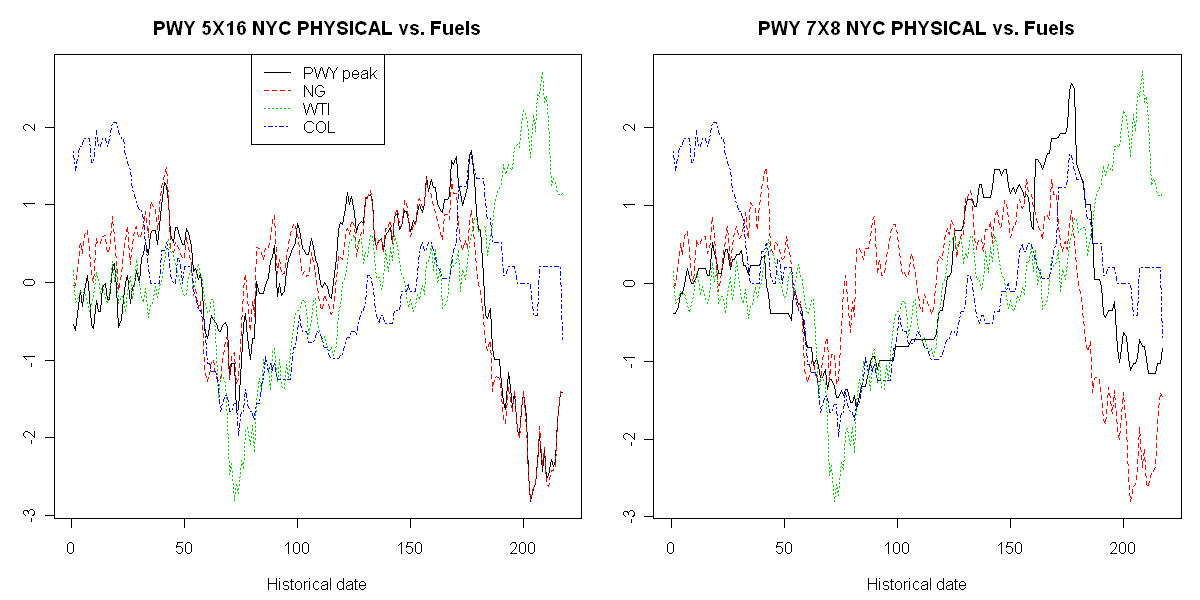
\includegraphics[width=6in, height=3in]{figures/pwy-fuel.png}
\caption{Major PWY peak and offpeak curves vs. Fuels, September 2007 contract.}
\label{pwy-fuel}
\end{figure}

Since the correlation between electricity and fuels depends on load,
they might show seasonalities. Figure \ref{pwy-fuel-corr} shows 
the correlation between electricity and fuels by contract month.
One can see for peak curve the correlation to NG is always high,
above 0.9 most of the time. The correlatino to COL and WTI were low
in the begining but climbed up quickly. 
For offpeak curve the correlation to NG and COL both started from around
0.6, and the corrlation to WTI started low. The correlations to all
three fuels show some seasonality with the correlation are lower
in early winter. 
\begin{figure}[htbp]
\centering
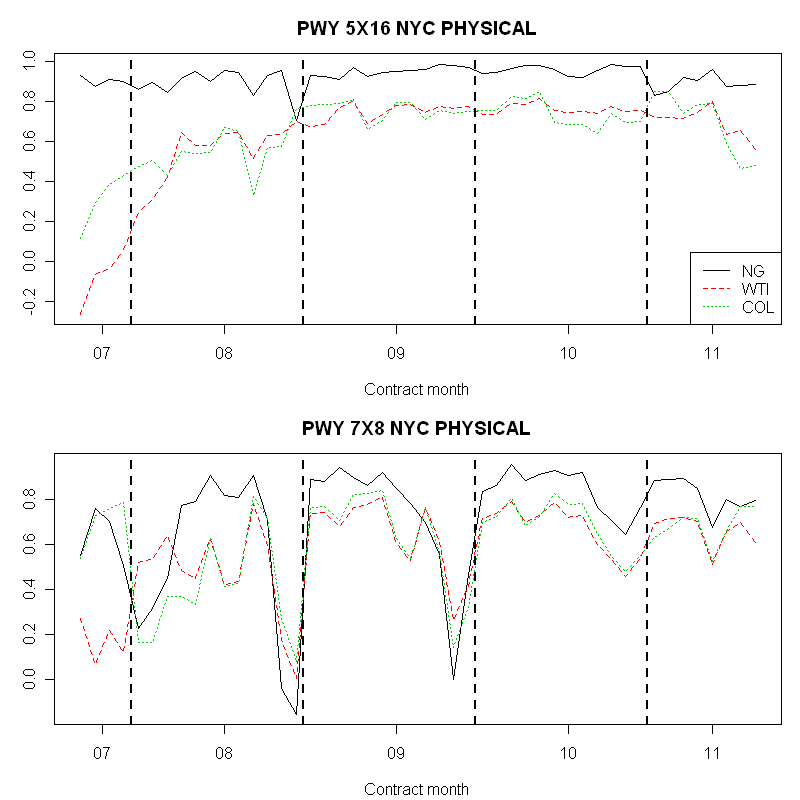
\includegraphics[width=3in, height=3in]{figures/pwy-fuel-corr.png}
\caption{Correlation between major PWY peak and offpeak curves vs. Fuels, 
for contract months over next four years.}
\label{pwy-fuel-corr}
\end{figure}


\subsection{Others}
There are many other markets including freight, emission. 
I did spend much time on them so the description on those curves
will be skipped. Since the scale of those data is not very big,
I will simulate them all at once, market by market.

\subsection{Volatility}
We suspected that the volatility will increase when 
a contract approaching the maturity date. So we 
studied the volatility of some curves. 
Figure \ref{ng-exch-vol} shows the daily log returns of 
four expired contracts for NG EXCHANGE. It's not obvious 
that the volatility changes change a long with time.
\begin{figure}[htbp]
\centering
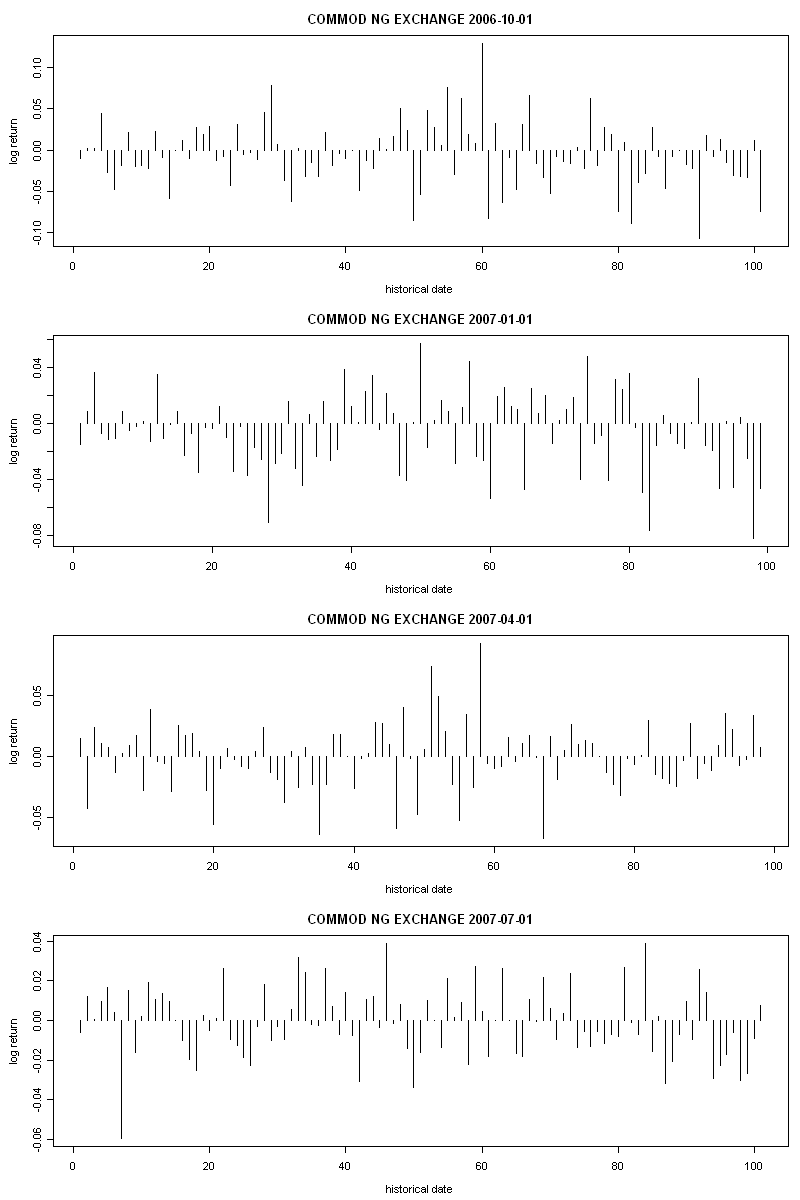
\includegraphics[width=6in, height=8in]{figures/ng-exch-vol.png}
\caption{Daily log returns of four expired contracts for NG EXCHANGE}
\label{ng-exch-vol}
\end{figure}

Figures \ref{pwy-offpeak-vol} and \ref{pwy-peak-vol} 
show the same plots for one offpeak and one peak curves for PWY. 
Interestingly the volatilities seem to increase when approaching maturity
for January and July contracts, but not so for April and October contracts.
\begin{figure}[htbp]
\centering
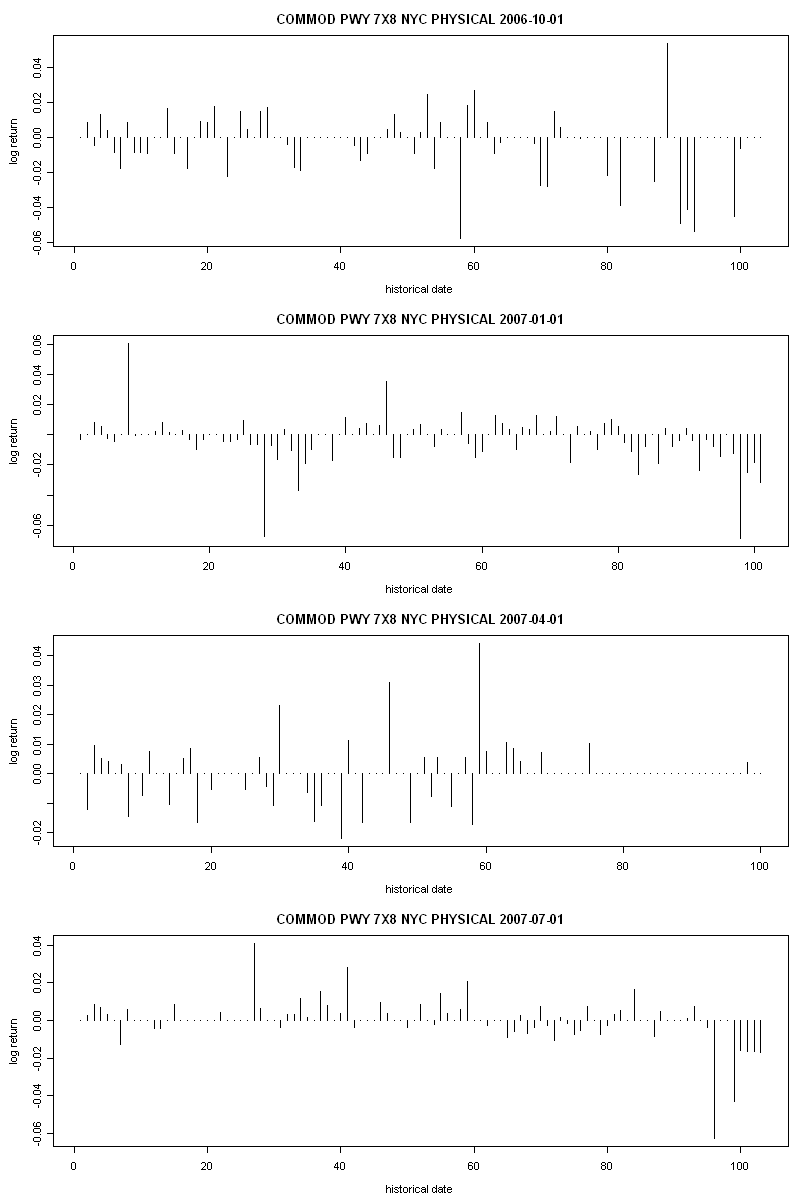
\includegraphics[width=6in, height=8in]{figures/pwy-offpeak-vol.png}
\caption{Daily log returns of four expired contracts for PWY 7X8 NYC PHYSICAL}
\label{pwy-offpeak-vol}
\end{figure}

\begin{figure}[htbp]
\centering
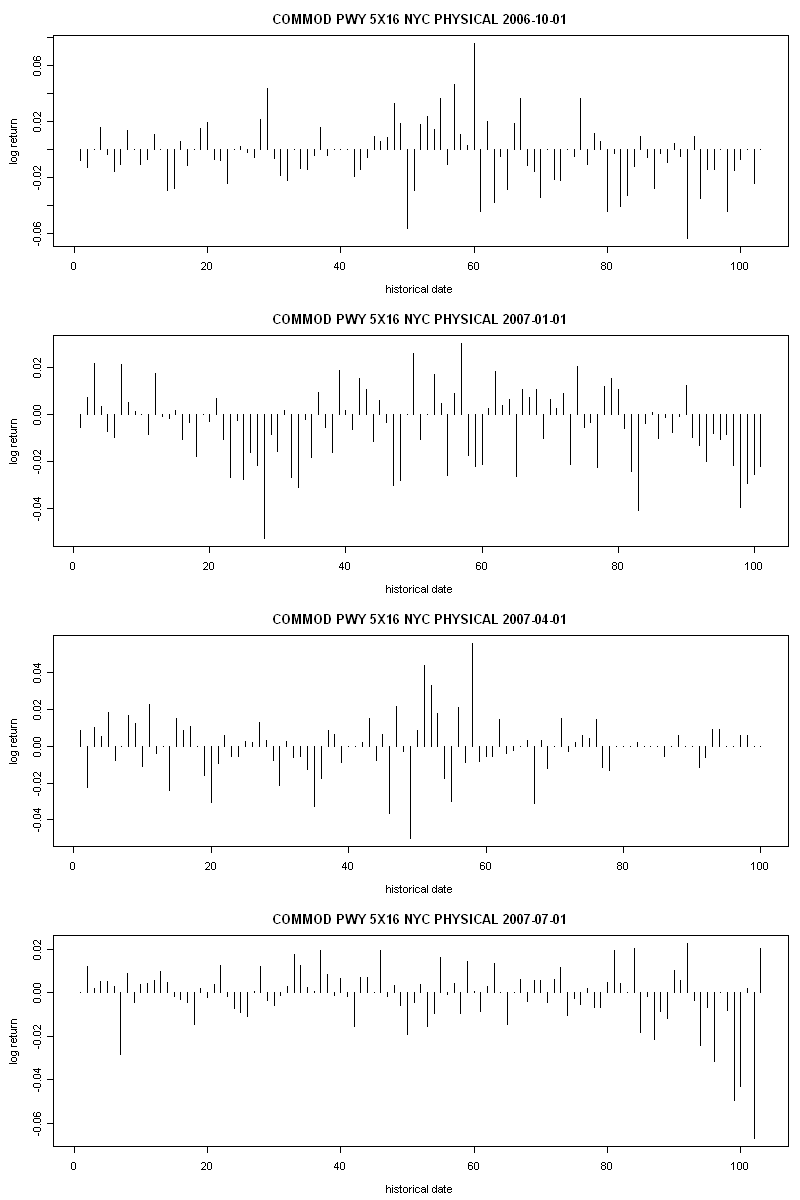
\includegraphics[width=6in, height=8in]{figures/pwy-peak-vol.png}
\caption{Daily log returns of four expired contracts for PWY 5X16 NYC PHYSICAL}
\label{pwy-peak-vol}
\end{figure}

We did the same plots for two PWJ curve, one peak and one offpeak,
as shown in Figures \ref{pwj-offpeak-vol} and \ref{pwj-peak-vol}.
We observed a similar pattern as in PWY curves. This is a interesting 
finding, which might suggest the volatility changes show some 
seasonality. Maybe during peak seasons there are many unpredictable
factors and the traders made wrong decision more often. 
We will have to explore more curves to make a reasonable claim.
Modeling volatility is difficult and one have to make some 
parametric assumptions. Throughout this work I made an assumption that
the volatilities didn't change along with time.
\begin{figure}[htbp]
\centering
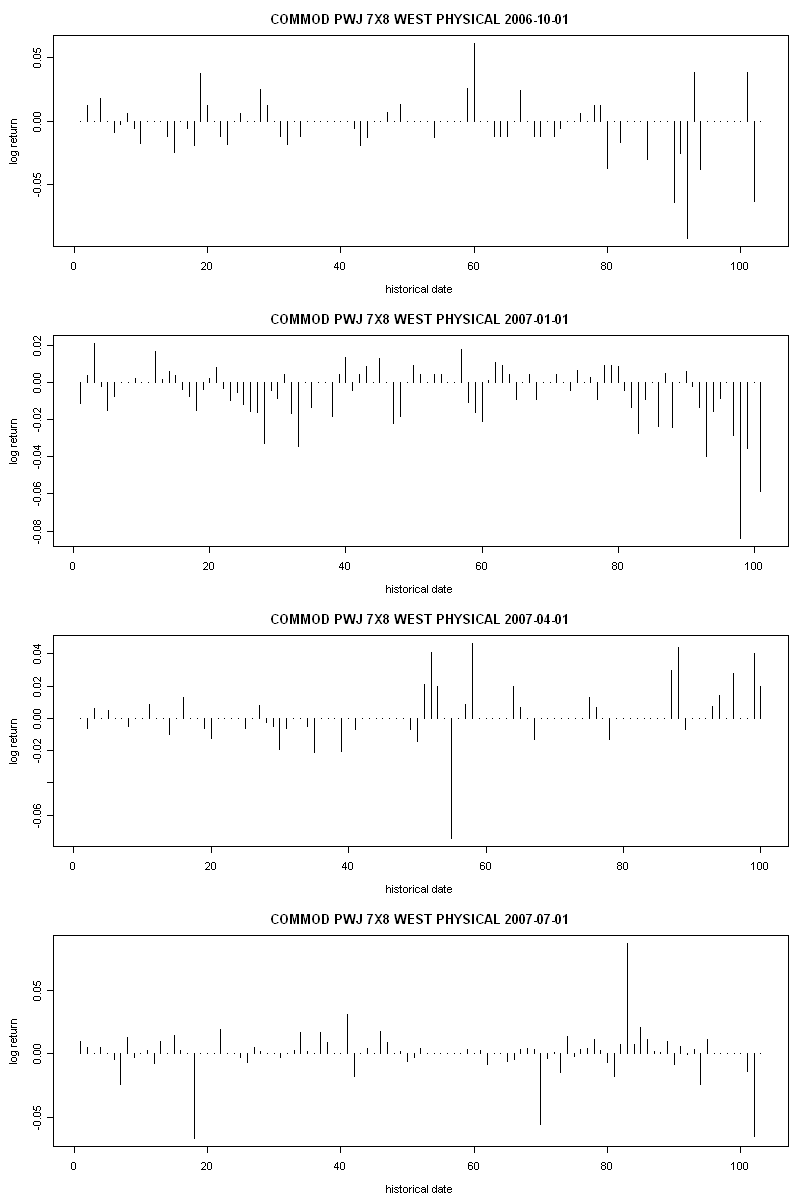
\includegraphics[width=6in, height=8in]{figures/pwj-offpeak-vol.png}
\caption{Daily log returns of four expired contracts for PWJ 7X8 DOMHUM PHYS}
\label{pwj-offpeak-vol}
\end{figure}

\begin{figure}[htbp]
\centering
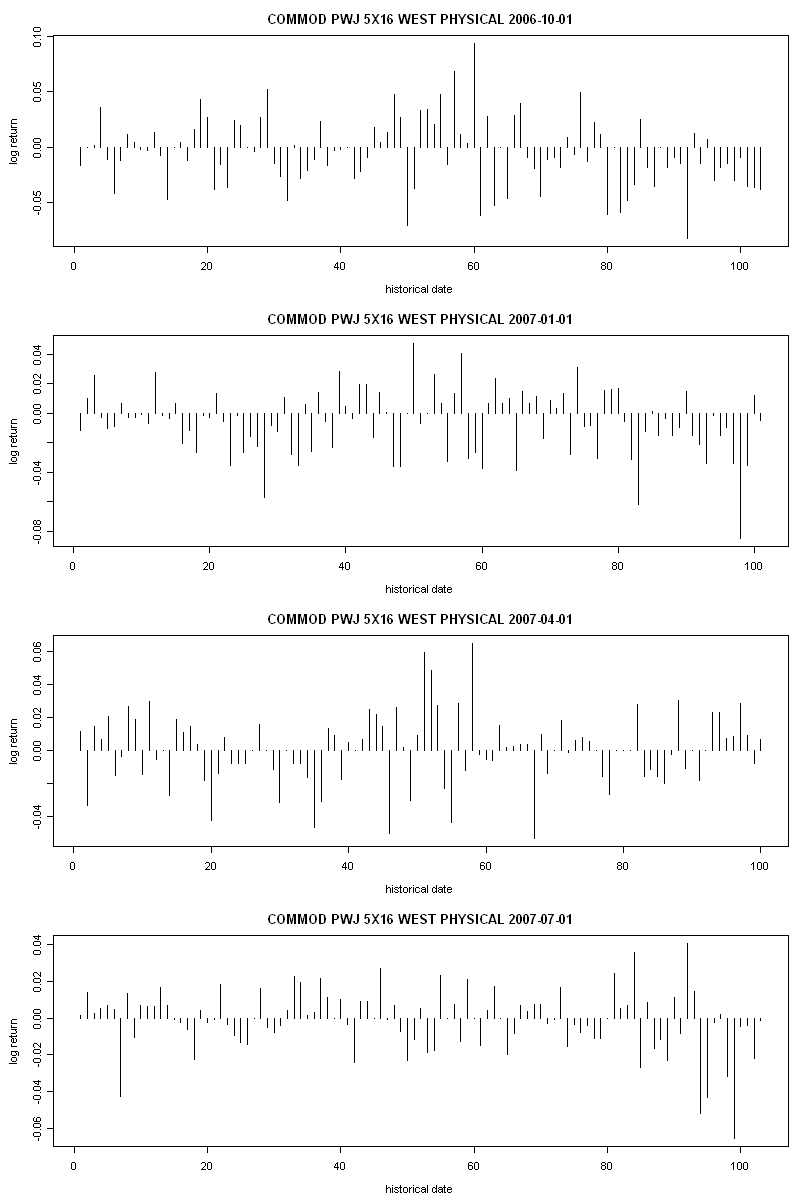
\includegraphics[width=6in, height=8in]{figures/pwj-peak-vol.png}
\caption{Daily log returns of four expired contracts for PWJ 5X16 DOMHUM PHYS}
\label{pwj-peak-vol}
\end{figure}

